\chapter{Background}

This chapter aims to explain the basic concepts that are the most important to the work in this thesis.


% -------------------------------------------------------
% -------------------------------------------------------
% ----------------- Machine Learning --------------------
% -------------------------------------------------------
% -------------------------------------------------------
\section{Machine Learning}

The following sections will define the term 'Machine Learning'. 
It will describe some various ways that machine learning can be applied.



\subsection{What is machine learning?}

As a term, 'Machine Learning' is a subcategory if the umbrella term 'Artificial Intelligence'.
It is proposed as an alternative to traditional algorithms. 
Machine Learning takes a set of input (training) data, and attempts to reason about some quality of the input, 
without the author of the program explicitly telling the program what quality of the input data we are interested in reasoning about.
Instead, the author provides the Machine Learning model with their optimal target for the given input,
and the model must attempt to generalize over, and design its own algorithm to fit the target.

This approach has become useful in problems where discovering the target based on the model input becomes computationally intractible,
or when the target cannot be determined as a direct consequence of the input. 
An example of such a problem is sentiment analysis of text input. 
Given the sentence 'The nice boy made fun of the kind girl', 
it is difficult to design rules which can capture the sentiment of the sentence.
On one hand, the words 'nice', 'fun', and 'kind' indicate this sentence may have a positive sentiment.
In reality, our ability to reason tells us that this is not the case, and the sentence is of a negative nature.

Machine Learning is deeply rooted in Bayesian Statistics. (Noen gode setninger om bayes. Gjerne bayes teorem? Ikke mer enn et avsnitt. Dette er en AI-oppgave, ikke en statistikk-oppgave.)


\subsection{Linear Regression}

As a first study in the implementation of machine learning, we look at linear regression.
To explan linear regression, we view an example in a two dimensional, euclidean space.
We are given a set of input data values $ X $ . Each input value $ x_i \in X $ has a corresponding output value $ y_i \in Y $.
We can plot each input value, and its corresponding output value as coordinates.


To describe a function that best maps the given inputs with their related outputs, 
we introduce two variables $ w_0 $ and $ b_0 $. We define a function to map our input values to their corresponding output.

\[
        f(x) = w_0x + b \tag{2.1} \label{linreg}
\]

We also introduce some measure of how well our function $ \eqref{linreg} $
maps our input to our output. As we tune our function variables $ w_0 $ and $ b_0 $ to better map the input to its corresponding output,
the measure will decrease. There exists values for our variables $ w_0 $ and $ b_0 $  such that the measure defined in $ \eqref{mse} $ reaches its lowest possible value.
In this state, the function optimally maps the input data to with its corresponding output, given our function.

\[
    \mathbb{L} = \frac{1}{|X|}\sum_{i = 0}^{|X|} \big(y_i - f(x_i)\big)^2 \tag{2.2} \label{mse}
\]

Of course, the function defined in $ \eqref{linreg} $ is arbitrary. 
We can add or remove existing or additional function variables as we wish,
if we see that changing the function structure improves at mapping the input to the output.
 
\textbf{Referanse til taylor series expansion? Finn i Calculus bok}

\begin{figure}
    \centering
    \subfloat[\centering Input x values plotted against their corresponding y values]{{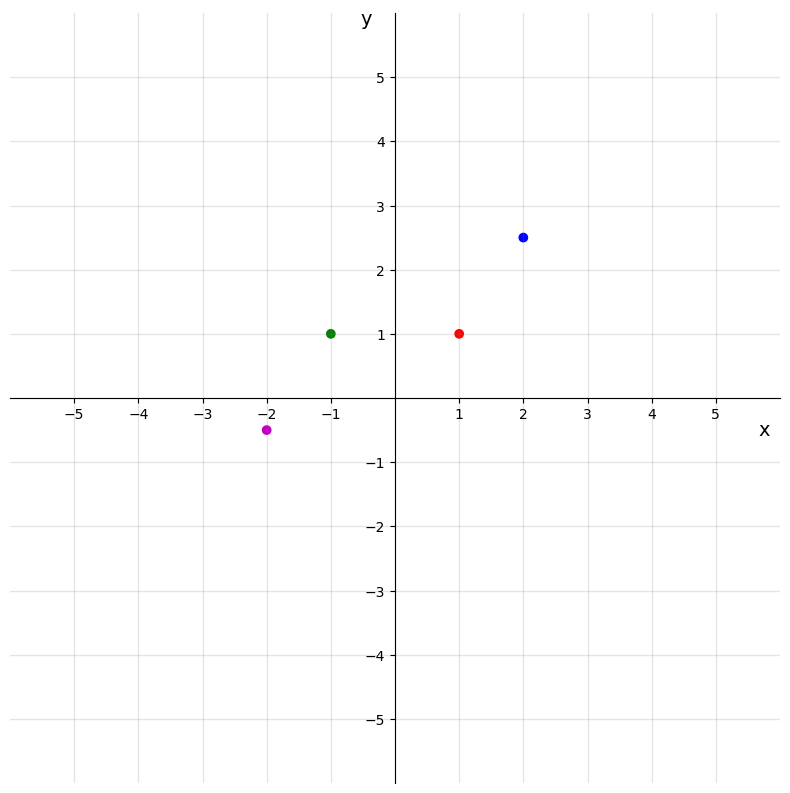
\includegraphics[width=7cm]{figures/background/linreg_input_illustrated.png} }}%
    \qquad
    \subfloat[\centering label 2]{{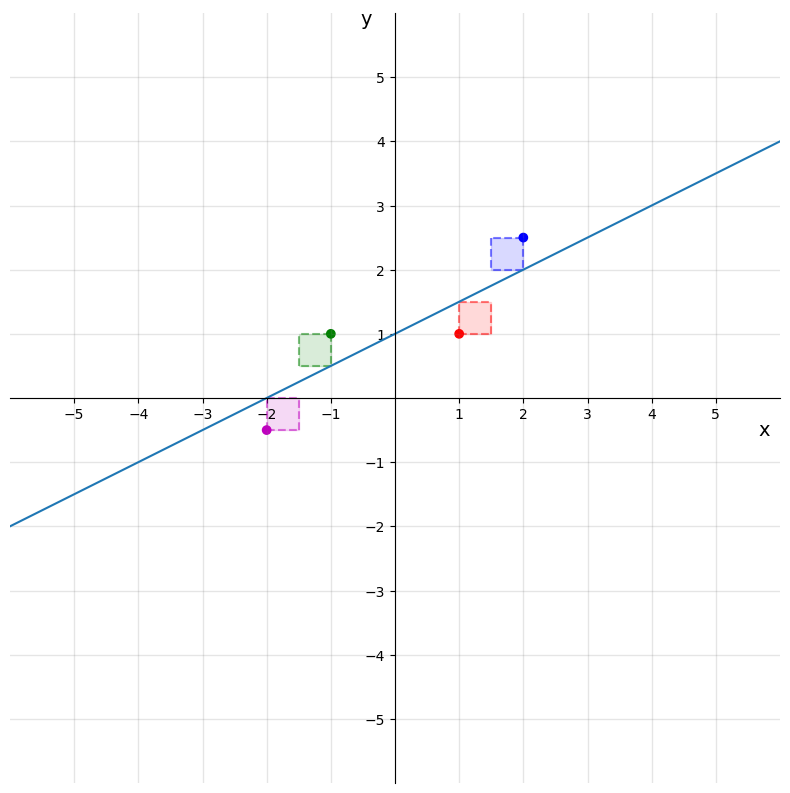
\includegraphics[width=7cm]{figures/background/MSE_illustrated.png}}}
    \caption{Linear regression illustrated}%
    \label{fig:linearRegression}%
\end{figure}



\subsubsection{Loss}

In the previous section, a measure of how 'wrong' a mapping of input points to their corresponding output points was defined.
In the litterature, this measure is referred to as the loss function. 
The loss function defined in $ \eqref{mse} $ is named 'Mean Squared Error Loss', 
due to the fact that it is defined by the mean of the squared difference between our function's predictions and the true values.

It is possible to define different loss functions. 
Different loss functions will interpret the performance of a functions mapping of the given input data to its corresponding output in different ways.
If we 

\[ 
    \mathbb{L} = \frac{1}{|X|}\sum_{i = 0}^{|X|} \sqrt{\big(y_i - f(x_i)\big)^2} \tag{2.2} \label{mae} 
\]





\subsection{Multi Layer Perceptron}
\subsection{Neural Networks}
underfitting and overfitting?
\subsubsection{Linear Layers}
\subsubsection{Activation functions}
\subsection{Backpropagation}
\subsection{Supervised and unsupervised learning}














% -------------------------------------------------------
% -------------------------------------------------------
% ---------------------- Graphs -------------------------
% -------------------------------------------------------
% -------------------------------------------------------
\section{Graphs}
\subsection{Nodes and Edges}
\subsection{Directed Acyclic Graphs}




% -------------------------------------------------------
% -------------------------------------------------------
% ---------------- Graph Neural Networks ----------------
% -------------------------------------------------------
% -------------------------------------------------------
\section{Graph Neural Networks}
\subsection{The Convolution Layer}
\subsection{Permutation invariance and equivariance}
\subsection{Attention and Message Passing}




% -------------------------------------------------------
% -------------------------------------------------------
% --------------- Gated Recurrent Units -----------------
% -------------------------------------------------------
% -------------------------------------------------------
\section{Gated Recurrent Units}
\subsection{Backpropagation Through Time}